\section{Notations and Definitions}

\begin{frame}[standout, plain, noframenumbering]
    Notations and Definitions

    % \medskip

    % \footnotesize
    % Sam Greydanus \quad Misko Dzamba \quad Jason Yosinski
\end{frame}


\begingroup
\small

\begin{frame}
    \frametitle{Manifolds and Vector Fields}

    \begin{itemize}
        \item $\mc{M}$ (state-space) denotes a manifold of finite dimension $n$.
        \item $f \in \mathfrak{X}(M)$ is a continuous vector field on $\mc{M}$.
        \item We assume that there exists a unique right maximally defined
        integral curve of $f$ starting at $x$.
        \item We also assume that this integral curve is defined on $[0,
        \infty]$.
        \[
            \varphi: [0, \infty] \times \mc{M} \rightarrow \mc{M}
        \]
        with 
        \begin{align*}
            \varphi(0, x) &= x, \\
            \varphi(t_1, \varphi(t_2,x)) &= \varphi(t_1+t_2, x).
        \end{align*}
        \item The semiflow $\varphi$ is the evolution function.
    \end{itemize}
\end{frame}


\begin{frame}
    \frametitle{Invariant and Stable Sets}

    \begin{definition}
        $\Omega \subseteq \mc{M}$ is called an \textsc{invariant set} if for all
        $x \in \Omega$ and $t \in \mathbb{R}_{\geq 0}$, $\varphi(t,x) \in
        \Omega$. If $\Omega = \{p\}$ is a singleton, then $\Omega$ is called and
        \textsc{equilibrium point} of the dynamical system $(\mc{M}, \varphi)$.
    \end{definition}

    \begin{definition}
        $\Omega \subseteq \mc{M}$ is \textsc{stable} if for \textit{every open
        neighborhood} $\mc{U} \subseteq \mc{M}$ of $\Omega$, \textit{there
        exists a neighborhood} $\mc{V} \subseteq \mc{M}$ of $\Omega$ such that 
        $\varphi(t, \mc{V}) \subseteq \mc{U}$ for all $t \geq 0$.

        An \textit{invariant set} $\Omega$ is asymptotically stable if

        \begin{itemize}
            \item $\Omega$ is stable,
            \item $\Omega$ is attractive, i.e., for all $x \in \Omega$, there
            exists an open neighborhood $\mc{N} \subseteq \mc{M}$ of $\Omega$
            such that for all $x \in \mc{N}$, $\varphi(t, x) \xrightarrow[]{t
            \rightarrow \infty} \Omega$.
        \end{itemize}
    \end{definition}
\end{frame}


\begin{frame}
    \frametitle{Domain (Region) of Attraction}

    \textit{The} domain of attraction is denoted by
    \[ \mc{A} = \{ x \in \mc{M}: \varphi(t,x) \rightarrow \Omega \text{ as } t
    \rightarrow \infty \}. \]

    $\Omega$ is said to be \textsc{globally} asymptotically stable if $\mc{N} =
    \mc{M}$.

    \begin{definition}
        The \textsc{Lie derivative} of $V: \mc{M} \rightarrow \mathbb{R}$ along
        $f \in \mathfrak{X}(\mc{M})$ is defined by 
        %
        \begin{align*}
            \mc{L}_fV: \mc{M} &\rightarrow \mathbb{R}, \\
            p &\mapsto \dd V_p (f(p)).
        \end{align*}
    \end{definition}
\end{frame}


\begin{frame}
    \frametitle{Lyapunov Function}

    \begin{definition}
        Let $\mc{K}$ be an invariant set of the dynamical system $(\mc{M},
        \varphi)$. A continuous function $V: \mc{A} \rightarrow \mathbb{R}_{\geq
        0}$ is a \textsc{Lyapunov function} if

        \begin{itemize}
            \item $V(x) > 0$ for all $x \in \mc{A} \backslash \mc{K}$,
            \item $V(x) = 0$ for all $x \in \mc{K}$,
            \item $V$ is proper, i.e., $V^{-1}(B)$ is compact for all compact
            subset $B \subseteq \mathbb{R}_{\geq 0}$,
            \item $V$ is strictly decreasing along orbits of $\varphi$, i.e.,
            \vspace{-1mm}
            \[ V \circ \varphi(t,x) < V(x), \] \vspace{-1mm} for all $t > 0$ and
            $x \in \mc{A} \backslash \mc{K}$.

            If $V$ is differentiable, this condition may be replaced by
            %
            \[ \mc{L}_fV(x) < 0. \]
        \end{itemize}
    \end{definition}
\end{frame}


\begin{frame}
    \frametitle{(Nondegenerate) Critical Points}

    \begin{definition}
        Let $V: \mc{M} \rightarrow \mathbb{R}$ be a smooth function. A
        \textsc{critical point}, $p \in \mc{M}$, of $V$ is a point where the
        differential \[ \dd V_p: T_p\mc{M} \rightarrow \mathbb{R} \] has rank
        zero, i.e., in any local coordinate system $\{x_i\}_{1}^n$, one has
        $\pd{V}{x_i}(p) = 0$ for all $i = 1, \ldots, n$.
    \end{definition}

    \begin{definition}
        A critical point $p$ is \textsc{nondegenerate} if the Hessian $H_p(V)$
        is a nondegenerate bilinear form, i.e., if any coordinate system, the
        Hessian matrix \[ \left( \frac{ \partial^2 V }{ \partial x_i \partial
        x_j } \right)_{1 \leq i,j \leq n} \] is nondegenerate.
    \end{definition}
\end{frame}


\begin{frame}
    \frametitle{Nondegenerate Critical Points}

    \begin{definition}
        The dimension of the subspace of $T_p\mc{M}$ on which $H_p(V)$ is
        negative definite is called the \textsc{Morse index} of $V$ at $p$,
        denoted by $\text{ind}(V, p)$.
    \end{definition}

    \begin{definition}
        A $C^2$ function $V: \mc{M} \rightarrow \mathbb{R}$ is a \textsc{Morse
        function} if all its critical points are nondegenerate.
    \end{definition}

    \begin{definition}
        The \textsc{(sub)-level sets} of a function $V: \mc{M} \rightarrow
        \mathbb{R}$ are
        \begin{align*}
            \mc{M}_a &= V^{-1}\left( (-\infty, a] \right), \\
            \mc{M}_{a,b} &= V^{-1}\left( [a, b] \right). \\
        \end{align*}
    \end{definition}
\end{frame}


\begin{frame}
    \frametitle{Topological Definitions}

    \begin{itemize}
        \item A top. space is an \textsc{$n$-cell} if it is homeomorphic to
        $\mathbb{R}^n$.
        \item A top. space $X$ is \textsc{contractible} if it is
        \textit{homotopy equivalent} to the one-point space.
        \item A subspace $A$ of $X$ is called a \textsc{deformation retract} of
        $X$ if there exists a continuous function $ h: [0,1] \times X
        \rightarrow X $ such that for all $x \in X$, $a \in A$, 
        \begin{align*}
            h(0,x) &= x, \\
            h(1,x) &\in A, \\
            h(1,a) &= a.
        \end{align*}
        \item The $k^{\text{th}}$ \textsc{Betti number} of $\mc{M}$, denoted by
        $b_k$ is the rank of the $k^{\text{th}}$ homology group $H^k(\mc{M})$.
        \item The \textsc{Euler characteristic} of $\mc{M}$ is defined by
        \[ \chi(\mc{M}) = \sum_{i=1}^k (-1)^k b_k. \]
    \end{itemize}
\end{frame}

% \begin{frame}
%     \frametitle{Angular Velocity: The Fixed Axis Case}

%     \begin{columns}
%         \begin{column}{0.5\textwidth}
%             \begin{align*}
%                 \omega &= \dot{\theta}k, \\
%                 v &= \omega \times r.
%             \end{align*}
%         \end{column}
%         \begin{column}{0.5\textwidth}
%             \begin{figure}[bth]
%                 \centering
%                 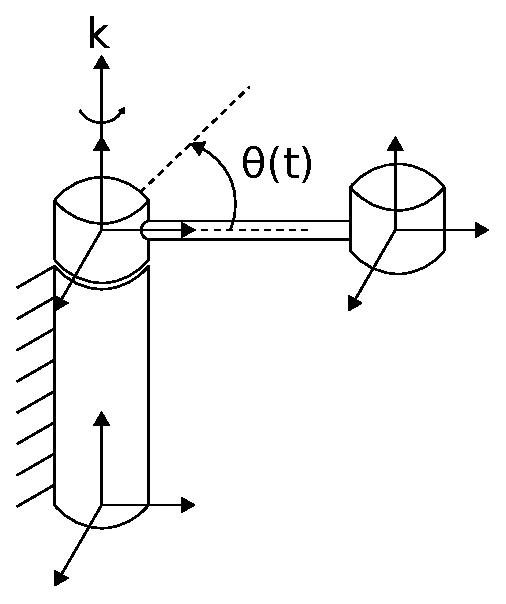
\includegraphics[width=0.5\textwidth]{figures/simple_rot.eps} 
%                 % \caption{\footnotesize Rotational motion of a one DoF manipulator.}
%             \end{figure}
%         \end{column}
%     \end{columns}

%     \begin{itemize}
%         \item In introductory dynamics courses, the computation of the linear
%         velocity $v$ is often the goal.
%         \item In our applications, we are interested in describing the motion of 
%         a moving frame:
%         \begin{itemize}
%             \footnotesize{
%             \item motion of the origin of the frame through space,
%             \item motion of the frame's axes.
%             }
%         \end{itemize}
%         \item For our purposes, the angular velocity will hold equal status with 
%         linear velocity.
%     \end{itemize}
% \end{frame}


% \begin{frame}
%     \frametitle{Angular Velocity: The Fixed Axis Case}
   

%     \begin{itemize}
%         \item The angular velocity is a property of the body-fixed coordinate
%         frame.
%         \item Angular velocity is \textit{not} a property of individual points.
%         \item Individual points may experience a \textbf{linear velocity} that 
%         is induced by an angular velocity, but it makes no sense to speak of a 
%         point itself rotating.
%         \item Thus, in equation~\eqref{eq:lin_vel_fixed}, $v$ corresponds to the 
%         linear velocity of a point, while $\omega$ corresponds to the angular 
%         velocity associated with a rotating coordinate frame.
%     \end{itemize}
% \end{frame}


% \begin{frame}
%     \frametitle{Angular Velocity: The Fixed Axis Case}

%     \begin{itemize}
%         \item In the fixed axis case, the problem of specifying angular 
%         displacements is really a planar problem
%         \begin{itemize}
%             \footnotesize{
%             \item each point traces out a circle,
%             \item every circle lies in a plane.
%             }
%         \end{itemize}
%         \item It is tempting to use $\dot{\theta}$ to represent the angular 
%         velocity.
%         \item However, this choice, does not generalize to the three-dimensional 
%         case.
%         \item We will develop a more general representation for angular velocities.
%         \item This will be analogous to our development of rotation matrices.
%         \item The key tool in this development is the skew-symmetric matrix.
%     \end{itemize}
% \end{frame}


\endgroup